CPU speeds are usually measured by timing the execution time of programs. Since
a computer program is just a collection instructions, the speed of the CPU is
determined by how fast it can process each instruction.
Every CPU has a clock, which ticks at a given rate. For every tick, a new
instruction is executed. This clock ensures that all instructions "flow" through
the processor without problems, and that the electrical components, such as the
ALU or the control-unit, can manage to carry out their tasks in that time.
Naturally, electrical engineers have pushed the limits of the circuits to manage
the highest clock rate. The clock rate of the very first processors was measured
in hertz and kiloHertz (kHz), but most modern desktop CPUs reach in multiple
GigaHertz (GHz)\cite{wiki:clock_rate}. However, even with those speeds, the
demand for faster processing units is ever-growing, and other techniques to speed-up
the execution are used.\\
One of those techniques is pipelining, which separates the circuit into multiple
stages, much like the assembly lines in factories. In such factories, workers
have their own station at the assembly line, do a specific task repeatedly, and
forward it down the line. This greatly increases the throughput of a factory and
decreases the labor need.
In MIPS, this idea is implemented by separating the processor into 5 stages\cite{COD5}:
\begin{itemize}
	\item Instruction Fetch (IF)
Fetches the next instruction.

	\item Instruction Decode (ID)
Reads the instruction, sets the appropriate control flags, reads the relevant
registers and sends the data to the next stage.

	\item Execute
Executes the instruction. This is typically done by the ALU with the appropriate
operation supplied.

	\item Memory Access
All operations on memory happen here. This stage either loads a memory address
or stores a value at an appropriate address.

	\item Write Back
Writes the results to the CPU registers.
\end{itemize}
Each of these stages will naturally use less time than all of them combined, and
since the clock is shared in all stages, it is set to the slowest stage in the
pipeline.\\
Not only do we have faster tick rate on our clock, but we are also able to
perform multiple operations concurrently. Figures \ref{fig:single_cycle_time}
and \ref{fig:pipeline_time} show the timing of each instruction, and how
pipelining might improve the whole process.
\begin{figure}[H]
        
\includegraphics{pipeline/single_cycle.eps}
        \label{fig:single_cycle_time}
\end{figure}
\begin{figure}[H]
        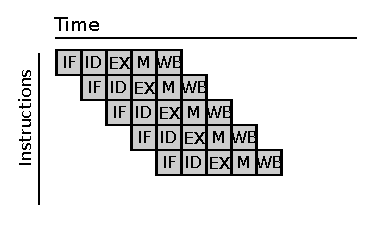
\includegraphics{pipeline/pipeline.eps}
        \label{fig:pipeline_time}
\end{figure}


\subsection{Design of the MIPS32 Pipeline}
The advantages of a pipelined design does not come without a price. Although
the single-cycle implementation of the processor is very similar to the
pipelined approach, it has its fair sets of challenges. The main problem with
executing instructions concurrently is that the instructions will often rely on
the result of the previous instructions. These situations are referred to as
hazards.

\subsubsection{Data Hazard}
Data hazards mainly occur when an instruction cannot continue, because it must
wait for the result from an earlier instruction. Suppose a program wants to
calculate the sum of 4 integers:
$$A = A + B + C + D$$
In MIPS32 assembly, this would be written as:
\begin{lstlisting}
# t0 = A, t1 = B, t2 = C, t3 = D
add $s0, $t0, $t1 	# s0 = A + B
add $s1, $t2, $t3	# s1 = C + D
add $v0, $s0, $s1
\end{lstlisting}

Here, the first two instruction will have no trouble executing, as they do not
share any source or destination registers. The third instruction however, will
not be able to fetch the updated values. When it is in the ID stage, where it decodes the
register \texttt{s0} and \texttt{s1} values, the previous instructions are
still in the pipeline, in the EX and MEM stage! These instructions have not
written back their results in the appropriate registers, and so, instruction 3
cannot fetch the correct value of s0 and s1, unless it waits 3 clock cycles.


